\documentclass{beamer}
\mode<presentation>
{
\usepackage{dis-template}
}
\usepackage{listings}
\usepackage{hyperref}

\graphicspath{{slides/}} % TODO: eliminate this hack, necessary because scons builds at repository root

%---------------------------------------------------------------------
\titlepageinit{5}{PCB Peer Review}{18 \& 19 Feb 2015 (Week 5)}
%---------------------------------------------------------------------
\begin{document}
%---------------------------------------------------------------------
\begin{frame}
\titlepage

\setcounter{tocdepth}{1}
\tableofcontents
\end{frame}

% LAB PREPARATION
% Print out checklists??

%---------------------------------------------------------------------
\section{PCB Peer Review} % [?? mins]
%---------------------------------------------------------------------
\begin{frame}
\centering \huge PCB Peer Review
\end{frame}

%---------------------------------------------------------------------
\subsection{Activity}

\begin{frame}
\frametitle{PCB Peer Review}
\begin{columns}[t]
\column{0.646\textwidth}
\begin{itemize}
  \item Why peer review?
  \begin{itemize}
    \item Get a fresh perspective on your board to catch bugs you've missed
    \item Get a new opinion from someone with a different background
    \item Facilitate transfer of knowledge
  \end{itemize}
  \item Things to look for in your peer reviews:
  \begin{itemize}
    \item Schematic style: messiness hides bugs!
    \item Circuit safety and spec check
    \item Layout sanity: DRC violations, don't design for minimums
    \item Really, anything that looks off
  \end{itemize}
\end{itemize}

\column{0.323\textwidth}
\begin{figure}
  \centering
  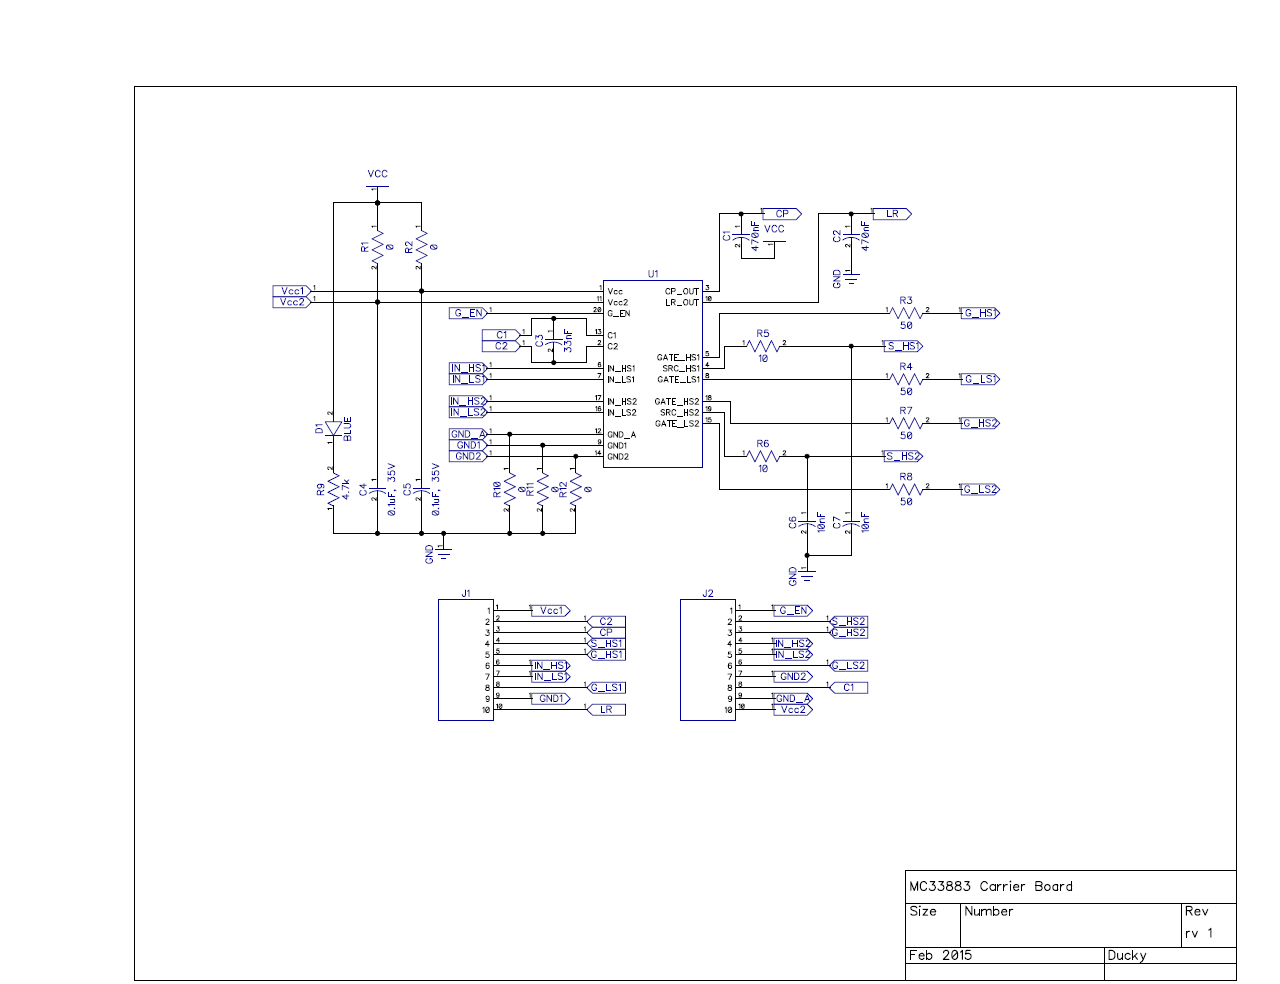
\includegraphics[width=1.0\columnwidth]{images-dis5/mc33883-schematic} \\
  Hopefully a fairly readable schematic
\end{figure}
\end{columns}
\end{frame}

\begin{frame}
\frametitle{PCB Peer Review}
\centering
Pair up with another team \\
{\tiny (or another two teams, if you're in an odd group of three)} \\
\hfill \\
Bring up the PCB Peer Review Checklist \\
{\tiny (\url{www-inst.eecs.berkeley.edu/~ee192/sp15/docs/dis5-pcbchecklist.pdf})} \\
{\tiny but feel free to add additional criteria as you want} \\
You'll have 30 minutes to review each other's boards \\
{\tiny (so about 15 minutes per team in a group)} \\
\hfill \\
Note anything you really liked about the boards you reviewed \\
{\tiny as well as pitfalls others should know and avoid} \\
\hfill \\
We'll discuss as a class after you're done in groups
\end{frame}

%---------------------------------------------------------------------
\section{Fabrication Data} % [?? mins]
%---------------------------------------------------------------------
\begin{frame}
\centering \huge PCB Fabrication Data
\end{frame}

%---------------------------------------------------------------------
\subsection{Gerbers}

\begin{frame}
\frametitle{Gerbers}
\begin{columns}[t]
\column{0.646\textwidth}
{\centering no, it's not baby food... \\}
\begin{itemize}
  \item The Gerber format (RS-274X) is a bi-level (2 ``colors'') vector image format
  \begin{itemize}
    \item De-facto standard for PCB layer data
  \end{itemize}
  \item The layers we're interested in are:
  \begin{itemize}
    \item top / bottom copper
    \item top / bottom silkscreen
    \item top / bottom soldermask (negative image)
    \item board outline
    \item drill file
  \end{itemize}
  \item You should export these from your design tool for submission to the board house
\end{itemize}

\column{0.323\textwidth}
\begin{figure}
  \centering
  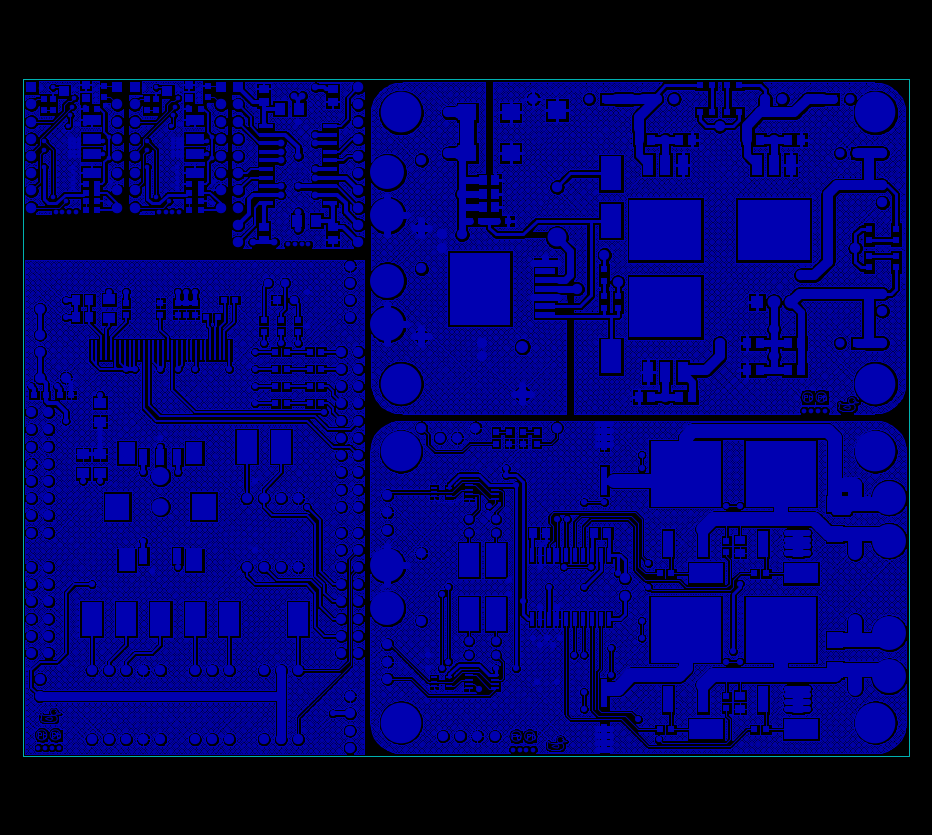
\includegraphics[width=0.75\columnwidth]{images-dis5/refcar-top} \\
  Top Copper Gerber \\
  \hfill \\
  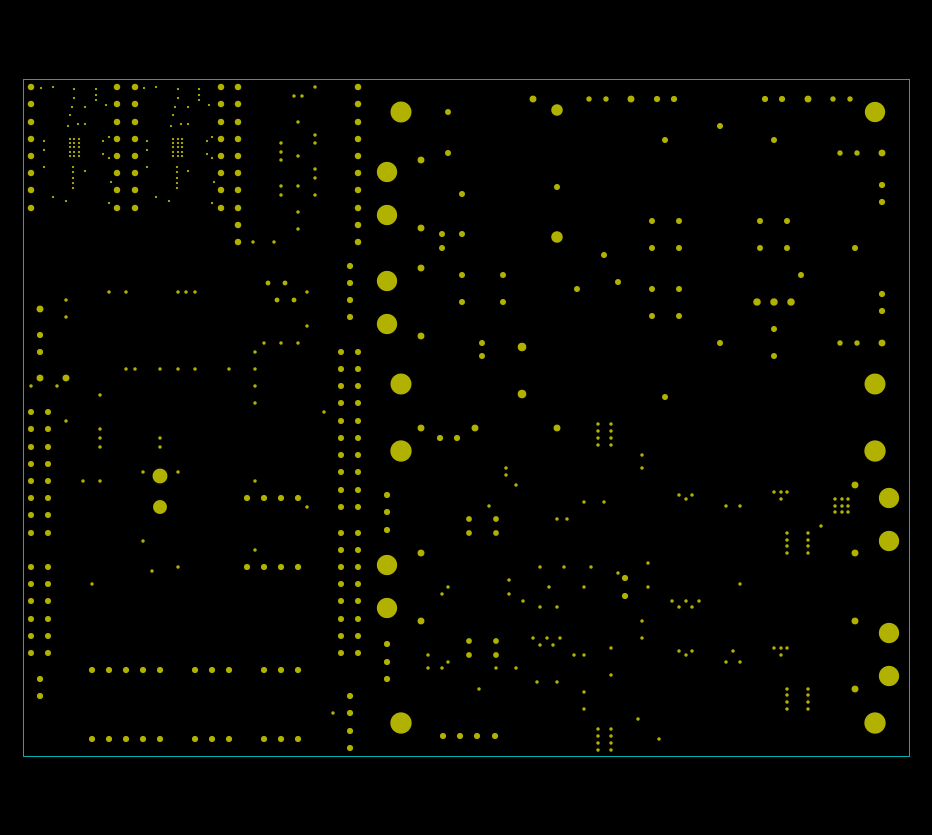
\includegraphics[width=0.75\columnwidth]{images-dis5/refcar-drill} \\
  N/C Drill file
\end{figure}
\end{columns}
\end{frame}

%---------------------------------------------------------------------
\subsection{DRC / DFM Checks}

\begin{frame}
\frametitle{InstantDFM}
\begin{columns}[t]
\column{0.646\textwidth}
\begin{itemize}
  \item DRC: Design Rules Check \\
  DFM: Design for Manufacturability
  \begin{itemize}
    \item or, can the board house make it and expect it to come out working
    \item These typically check for minimum feature sizes (trace width / spacing, hole size)
    \item If it fails, don't expect a functional board
  \end{itemize}
  \item Bay Area Circuits has a online DFM tool: (\url{instantdfm.bayareacircuits.com})
  \begin{itemize}
    \item Run your Gerbers through it to ensure it's within limits for fabrication
  \end{itemize}
\end{itemize}

\column{0.323\textwidth}
\begin{figure}
  \centering
  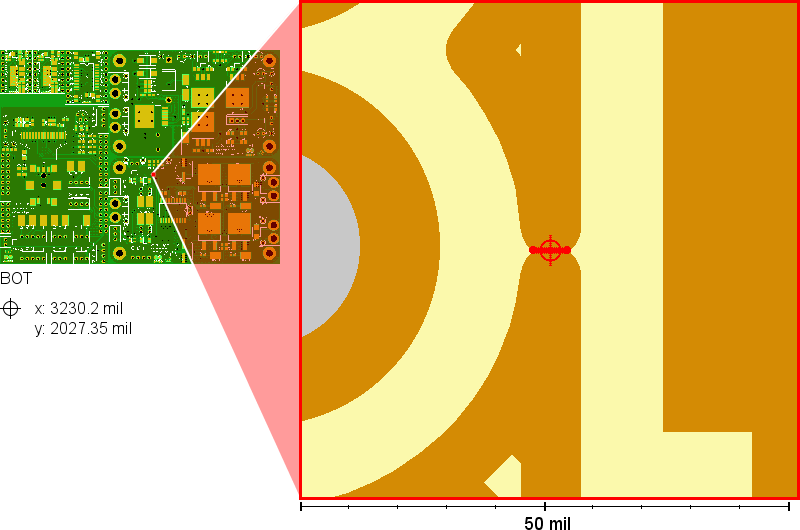
\includegraphics[width=1.0\columnwidth]{images-dis5/refcar-instantdfm} \\
  InstantDFM showing minimum trace width
\end{figure}
\end{columns}
\end{frame}

%---------------------------------------------------------------------
\subsection{bCourses Design Submission}
\begin{frame}
\frametitle{Deadlines and Submissions}
\begin{columns}[t]
\column{0.646\textwidth}
\begin{itemize}
  \item You get a 4"x6" board area
  \begin{itemize}
    \item See the Piazza post for exact specs
  \end{itemize}
  
  \hfill \\
  \item Submit everything as a .zip on bCourses
  \item Friday, 6pm: Design files for review by course staff
  \begin{itemize}
    \item We will check over your schematic and layout for obvious errors and return comments within 24 hours
  \end{itemize}
  \item Sunday, 6pm: Final Gerbers due
  \begin{itemize}
    \item This is what gets sent to the board house.
    \item Watch your email carefully - we will do a quick spot check - be prepared to fix errors FAST.
  \end{itemize}
\end{itemize}

\column{0.323\textwidth}
\vspace{20mm} \\
{\centering I don't think a bCourses screenshot would be helpful here}
\end{columns}
\end{frame}

%---------------------------------------------------------------------
\section{Summary} % [?? mins]

\begin{frame}
\frametitle{Summary}
Summary
\begin{itemize}
  \item Do design reviews so others can catch bugs that you won't!
  \item Generate Gerber fabrication data for your boards for submission
  \item Verify your designs through InstantDFM
\end{itemize}

\hfill \\
Parts Handout
\begin{itemize}
  \item Get a BlueSMiRF (Bluetooth serial terminal)
  \begin{itemize}
    \item this is how you \texttt{printf} on a moving platform
  \end{itemize}
  \item Get an encoder kit (board + S6986 + find a LED)
\end{itemize}

\hfill \\
Checkoff Reminders
\begin{itemize}
  \item Avoid alligator clip leads for your motor drivers. Your circuit should begin to resemble what would go on your car - make nice connectors with nice wiring which you can re-use when boards come in.
\end{itemize}
\end{frame}

\end{document}
